\section{Modal Approximation}  %    S    S    S    S    S    S    S    S    S
The following example represents a problem in linear regression. A sequence of $m$ data points $\paren{x_{k}, T_{k}}$,  $\kto{m}$  is recorded. The goal is to find the best approximation to a straight line. The \emph{trial function} is
  \begin{equation*}   %  =   =   =   =   =
    T(x) = a_{0} + a_{1} x .
    \label{eq:lr trial}
  \end{equation*}
The residual errors are the difference between the measurements and predictions:\\
  \begin{equation*}   %  =   =   =   =   =
      \text{residual error}_{k} = \underbrace{\text{measurement}_{k}}_{T_{k}} - \underbrace{\text{ prediction}_{k}}_{T(x_{k})}
  \end{equation*}
Formally, the residual error is
  \begin{equation*}   %  =   =   =   =   =
    r_{k} = T_{k} - T(x_{k}), \quad \kto{m}.
  \end{equation*}
From this springs the \emph{merit function}, the target of minimization,
  \begin{equation}   %  =   =   =   =   =
  \begin{split}
    M(a) 
      &= \sum_{k=1}^{m} r_{k}^{2} \\
      &= \sum_{k=1}^{m} \paren{\text{measurement}_{k} - \text{prediction}_{k}}^{2} \\
      &= \sum_{k=1}^{m} \paren{T_{k} - T\paren{x_{k}}}^{2} \\
      &= \sum_{k=1}^{m} \paren{T_{k} - a_{0} - a_{1} x_{k}}^{2}
    \label{eqn:merit}
  \end{split}
  \end{equation}
The least squares solution $a_{LS}$ is defined as 
  \begin{equation*}   %  =   =   =   =   =
    a_{LS} = \lst{a \in \cmplx{2} \colon \normts{T(x_{k}) - a_{0} - a_{1} x_{k}} \text{ is minimized} }.
  \end{equation*}
Colloquially, the least squares solution is the set $a$ of complex pairs such that the square of the norm $\normts{T(x_{k}) - a_{0} - a_{1} x_{k}}$ is minimized.

The solution set satisfies
  \begin{equation}   %  =   =   =   =   =
    \nabla M( a )|_{a_{LS}} = 0 .
    \label{eq:gradient lr}
  \end{equation}

\section{Bevington Example}  %    S    S    S    S    S    S    S    S    S

To provide a common reference, see the example in Bevington \cite[ch 6]{Bevington}. The data is summarized below in table \ref{tab:bevington data and results}. The problem involves temperature measurements $T_{k}$ made at position $x_{k}$ on a bar in contact with two heat baths (Dirichlet boundary conditions). A conceptualization is shown in figure \ref{fig:bar}. Arrowheads on the bottom show the nine locations where the temperature is measured.

In the ideal linear case, the temperature at the endpoints matches the temperature of the baths, $T(x=0 \text{ cm}) = 0^{\circ}$C and $T(x = 10 \text{ cm}) = 100^{\circ}$C which describes a line with intercept $a_{0} = 0^{\circ}$C and slope $a_{1} = 10^{\circ}$C/cm. Such an expectation is a crude quality measure, a ``sniff test''.

\begin{figure}[htbp] %  figure placement: here, top, bottom, or page
   \centering
   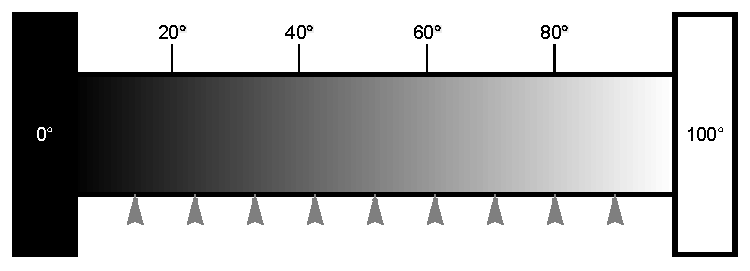
\includegraphics[ width = 3in ]{\pathgraphics "bevington classic"/bar} 
   \caption[Measuring the temperature of a bar.]{Measuring the temperature of a bar held between two constant-temperature heat baths.}
   \label{fig:bar}
\end{figure}

\subsection{Problem Statement}  %   SS   SS   SS   SS   SS   SS   SS   SS   SS   SS   SS   SS
Muddled conceptions are wellsprings for muddled execution. Success in dealing with complicated problems in least squares flows from being able to state the problem cleanly; a good practice is to start with a table specifying the problem of interest, such as table \ref{tab:bevington inputs}.

The first entry is the \emph{trial function} which defines the functional form to be applied to the data. As the name indicates, this function is an initial guess. Whether or not Nature has chosen this model remains to be seen.

The \emph{merit function} is created by inserting the trial function into \eqref{eqn:merit}. This function is the target of minimization and can provide a crude check on the solution. Given a candidate solution $a_{*}$, compute the value of $M(a_{*})$. The least squares solution has the property that $M(a_{*})$ has minimum value in the neighborhood of $a_{*}$. If the solution is perturbed, one must have $M(a_{*}) < M(a_{*} + \delta a)$. When you are developing and refining least squares algorithms, you may see that the computed solution $a_{*}$ changes. For overdetermined problems, the solution is unique and comparing the values of the merit function helps discriminate solutions. In a later section figure \ref{fig:bevington merit function} will demonstrate this behavior.

The \emph{measurements} define the quantities to be measured. It seems an obvious step, but more complex models may have ambiguities start here.

\emph{Results}, or fit parameters, define the quantities to be computed using the least squares algorithm. Together with the trial function, and the measurements, we now have a clear idea of what will be measured and what will be computed.

The \emph{residual error} specifies the difference between measurement and prediction at each point. A simple matter, apparent in the merit function, it is helpful to write it out, particularly for those who may be using the results and not intimate with the derivation.

The \emph{system matrix} describes the measurement apparatus and contains the dependent variables. In this example we have $m=9$ rows (measurements), $n=2$ columns (fit parameters) and a matrix rank $\rho = 2$ (full column rank and overdetermined).

The \emph{linear system} shows the application of the trial function to every measurement. It's a good idea to keep this image in mind.

The \emph{ideal solution} is an infrequent visitor which helps provide a rough measure of quality. Caution is required, though. The ideal solution typically represents a concatenation of miracles which Nature may avoid. In this example, the ideal solution assumes magic barriers which absorb no heat, a bar of exact length, thermometers with exact measurements, heat baths at exact temperatures, no interaction with the local environment, etc. The hope is that systematic effects will be negligible and random effects will have 0 mean.

  \begin{table}[h]  %  T A B L E
    \caption{Problem statement for linear regression.}
    \begin{center}
      \begin{tabular}{lll}
        %
        \bf{trial function} & $T(x) = a_{0} + a_{1} x$ & $^{\circ}$C \\
        \bf{residual error} & $r_{k} = T_{k} - a_{0} - a_{1} x$ & $^{\circ}$C \\
        \bf{merit function} & $M(a) = \sum_{k=1}^{m}\paren{T_{k} - a_{0} - a_{1} x}^{2}$  & $\paren{^{\circ}\mathrm{C}}^2$\\
        \bf{measurements}   & $x_{k}$, $\kto{m}$ & position, cm \\
                            & $T_{k}$, $\kto{m}$ & temperature, $^{\circ}$C \\
        \bf{results}        & $a_{0} \pm \eps_{0}$ & intercept, $^{\circ}$C \\
                            & $a_{1} \pm \eps_{1}$ & slope, $^{\circ}$C / cm \\
                            %& \multicolumn{1}{c}{$\A{}$} & \multicolumn{1}{c}{$x$} & \multicolumn{1}{c}{$\A{}$} \\
        \bf{\# of measurements} & $m = 9$ & rows in $\A{}$ \\
        \bf{\# of parameters}   & $n = 2$ & columns in $\A{}$ \\
        \bf{system matrix}  & $\A{} \in \real{9 \times 2}_{2}$ \\
        \bf{linear system}  & $\mat{cc}{1 & x_{1}  \\ \vdots & \vdots \\ 1 & x_{m}} 
                               \mat{c}{a_{0} \\ a_{1}} = 
                               \mat{c}{T_{1} \\ \vdots \\ T_{m}}$ \\
        \bf{ideal solution} & $\mat{c}{a_{0}\\a_{1}} = \mat{c}{0\\10}$ \\
        \bf{input data}     & table \ref{tab:bevington data and results}
        %
      \end{tabular}
    \end{center}
  \label{tab:bevington inputs}
  \end{table}%

The next phase is to gather and record the data as shown in table \ref{tab:bevington data and results}. Discussion of significant digits in the input data is deferred.

\begin{table}[h]
	\caption{Raw data and results.}
	\begin{center}
		\begin{tabular}{rcc|rr@{.}l}
		  %
		  & \multicolumn{2}{c}{Input} &  \multicolumn{3}{c}{Output} \\
		  %
		  & (cm) & $(^{\circ}C)$ & $(^{\circ}C)$ & \multicolumn{2}{c}{$(^{\circ}C)$} \\
		  %
		  $k$ & $x_{k} $ & $T_{k}$ & $T\paren{x_{k}}$ & \multicolumn{2}{c}{$r_{k}$} \\\hline
		  %
			 1 & 1 & 15.6 & 14.2222 & --1 & 37778 \\
			 2 & 2 & 17.5 & 23.6306 &   6 & 13056 \\
			 3 & 3 & 36.6 & 33.0389 & --3 & 56111 \\
			 4 & 4 & 43.8 & 42.4472 & --1 & 35278 \\
			 5 & 5 & 58.2 & 51.8556 & --6 & 34444 \\
			 6 & 6 & 61.6 & 61.2639 & --0 & 336111 \\
			 7 & 7 & 64.2 & 70.6722 &   6 & 47222 \\
			 8 & 8 & 70.4 & 80.0806 &   9 & 68056 \\
			 9 & 9 & 98.8 & 89.4889 & --9 & 31111 \\
		  %
		\end{tabular}
	\end{center}
	\label{tab:bevington data and results}
\end{table}%

\subsection{\label{sec:normal I}Normal Equations via Calculus}  %   SS   SS   SS   SS   SS   SS   SS   SS   SS   SS   SS   SS
In \S 6.4, Bevington solves the problem by applying calculus to the final form in \eqref{eqn:merit}, effectively solving \eqref{eq:gradient lr}. Introducing the notation
  \begin{equation*}   %  =   =   =   =   =
       \partial_{j} M (a_{0}, a_{1}) = \frac{\partial M(a_{0}, a_{1})}{\partial a_{j}}
  \end{equation*}
the simultaneous equations to solve are
  \begin{equation}   %  =   =   =   =   =
    \begin{split}
       \partial_{0} M (a_{0}, a_{1}) = 0 , \\
       \partial_{1} M (a_{0}, a_{1}) = 0 .
    \label{eq:bev pde}
    \end{split}
  \end{equation}
These two differential equations spawn the linear system
\begin{equation*}
  \begin{split}
    &-2 \sum_{k=1}^{m} \paren{T_{k} - a_{0} - a_{1}x_{k}} \phantom{x_{k}} = 0, \\
    &-2 \sum_{k=1}^{m} \paren{T_{k} - a_{0} - a_{1}x_{k}} x_{k}  = 0.
  \end{split}
\end{equation*}
Distributing the summation operators creates a more revealing form  \\[-5pt]
  \begin{equation*}   %  =   =   =   =   =
  \begin{array}{lclclcl}
    \sum\limits_{k=1}^{m} T_{k}       & = & a_{0} \sum 1     & + & a_{1} \sum x_{k}, \\
    \sum\limits_{k=1}^{m} T_{k} x_{k} & = & a_{0} \sum x_{k} & + & a_{1} \sum x_{k}^{2}, 
  \end{array}
  \end{equation*}
where summation from 1 to $m$ is implied. (Therefore $\sum 1 = m$.) The minimization criteria are
now recast as the linear system
  \begin{equation}   %  =   =   =   =   =
      \mat{ll}{\sum 1 & \sum x_{k} \\ \sum x_{k} & \sum x_{k}^{2}}
      \mat{c}{ a_{0} \\ a_{1} } = 
      \mat{l}{\sum T_{k} \\ \sum T_{k} x_{k}}.
    \label{eq:modal matrix eq}
  \end{equation}

The solution can be written immediately. Defining the determinant
  \begin{equation}   %  =   =   =   =   =
    \Delta = m \sum x_{k}^{2} - \paren{\sum x_{k}}^{2},
    \label{eq:det}
  \end{equation}
the matrix inverse is
  \begin{equation}   %  =   =   =   =   =
    \mat{cl}{m & \sum x_{k} \\ \sum x_{k} & \sum x_{k}^{2}}^{-1} = \Delta^{-1} 
    \mat{lc}{\ps \sum x_{k}^{2} & -\sum x_{k} \\ -\sum x_{k} & m } .
    \label{eq:bevington matrix inverse}
  %\end{split}
  \end{equation}
The solution to equation \eqref{eq:modal matrix eq} is the matrix product
  % = =  e q u a t i o n
  \begin{equation*}
    \mat{c}{a_{0} \\ a_{1} } = \Delta^{-1}
    \bl{
    \mat{ll}{\ps \sum x_{k}^{2} & -\sum x_{k} \\ -\sum x_{k} & \ps \sum 1}
    \mat{l}{\sum T_{k} \\ \sum T_{k} x_{k}}
    },
    \label{eqn:bevington solution product}
  \end{equation*}
  % = =
  \begin{equation}
  \begin{split}
    a_{0} &= \Delta^{-1} \paren{\sum x_{k}^{2}\sum T_{k} - \sum x_{k}\sum T_{k} x_{k}}, \\
    a_{1} &= \Delta^{-1} \paren{m \sum T_{k} x_{k} - \sum x_{k}\sum T_{k}}.
  \label{eqn:bevington soln sum}
  \end{split}
  \end{equation}
The final results agree with Bevington's equations 6--17:

Bevington's \S 6--5 is a succinct explanation of error propagation. In short, measurements are inexact, therefore results will be inexact. The beauty of the method of least squares is that the error in the solution parameters can be expressed in terms of the error in the data. Measurements without uncertainties are incomplete measurements.

The computation chain begins with an estimate of the parent standard deviation which is based upon the total error:
% = =  e q u a t i o n
  \begin{equation*}
    s^{2} \approx \frac{\rtr{*}} {m-n}.
  \end{equation*}
% = =
Error contributions for individual parameters are harvested from the diagonal elements of the matrix inverse in \eqref{eq:bevington matrix inverse}:
\begin{equation*}
  \begin{split}
    %
    \eps_{0}^{2} &= \frac{r^{\mathrm{T}}r}{\Delta\paren{m-n}} \sum x_{k}^{2} \\
    \eps_{1}^{2} &= \frac{r^{\mathrm{T}}r}{\Delta\paren{m-n}} \sum 1 \\
    %
  \end{split}
  \label{eqn:bevington error terms}
\end{equation*}
  
\section{Numerical Results}  %    S    S    S    S    S    S    S    S    S

  \begin{table}[t]  %  T A B L E
    \caption{Results for linear regression.}
    \begin{center}
      \begin{tabular}{lll}
        %
        \bf{fit parameters} & $a_{0}$ & intercept, $^{\circ}$C \\
                            & $a_{1}$ & slope, $^{\circ}$C / cm \\
        \bf{solution function} & $T(x) = a_{0} + a_{1} x$ & $^{\circ}$C \\
        \bf{solution error} & $\eps_{T}^{2}(x) = \eps_{0}^{2} + x^{2} \eps_{1}^{2} + a_{1}^{2} \eps_{x}^{2} $ &$^{\circ}$C \\
        \bf{computed solution} & $\mat{c}{a_{0}\\a_{1}} = \mat{c}{4.8\\9.41} \pm \mat{c}{4.9\\0.87}$ \\
        \bf{ideal solution} & $\mat{c}{ \tilde{a}_{0} \\ \tilde{a}_{1} } = \mat{c}{0\\10}$ \\
        \bf{$\rtr{*}$} & $316.6$ \\
        \bf{curvature matrix $\wxi{*}$} & $\frac{1}{180}\mat{rr}{95 & \mg{-15} \\ \mg{-15} & 3 }$\\[5pt]
        \bf{problem statement} & table \ref{tab:bevington inputs} \\
        \bf{input data}        & table \ref{tab:bevington data and results} \\
        \bf{plots}          & figure \ref{fig:bevington soln v data}    & 1. data \& solution \\
                            & figure \ref{fig:bevington residuals}      & 2. residual errors \\
                            & figure \ref{fig:bevington merit function} & 3. merit function \\
        %
      \end{tabular}
    \end{center}
  \label{tab:bevington solution}
  \end{table}%

Results are stated in two forms. The first is an integer form free of numerical errors inherent in binary representations with finite length. This liberates one from trying to determine if errors are in the algorithm or in machine arithmetic. To aid debugging, intermediate results are also provided.

The second form represents the answer which would be provided to a customer: the fit parameters and associated errors quoted with the proper amount of significant digits.
 
\subsection{\label{sec:exact form}Exact Form}  %   SS   SS   SS   SS   SS   SS   SS   SS   SS   SS   SS   SS
Exact results for the fit parameters are error follow. The product matrix in \eqref{eq:modal matrix eq} is 
  \begin{equation*}   %  =   =   =   =   =
    \mat{cl}{m & \sum x_{k} \\ \sum x_{k} & \sum x_{k}^{2}} = \mat{rr}{ 9 & 45 \\ 45 & 285 },
  \end{equation*}
with determinant \eqref{eq:det}
  \begin{equation*}   %  =   =   =   =   =
    \Delta =  540.
  \end{equation*}
The inverse of this matrix, \eqref{eq:bevington matrix inverse}, is
  \begin{equation*}   %  =   =   =   =   =
    \mat{cl}{m & \sum x_{k} \\ \sum x_{k} & \sum x_{k}^{2}} ^{-1} = \Delta^{-1} \mat{rr}{ 285 & -45 \\ -45 & 9 }.
  \end{equation*}
The solution vector, \eqref{eqn:bevington soln sum}, is
  \begin{equation*}   %  =   =   =   =   =
      a = \mat{c}{a_{0} \\ a_{1}} = \frac{1}{360} \bl{\mat{c}{1733 \\ 3387}}.
  \end{equation*}
The residual error vector is 
% = =  e q u a t i o n
  \begin{equation*}
        r = \frac{1}{360}
          \mat{r}{-496 \\ 2207 \\ -1282 \\ -487 \\ -2284 \\ -121 \\ 2330 \\ 3485 \\ -3352},
  \end{equation*}
% = =
making the total error
% = =  e q u a t i o n
  \begin{equation*}
        \rtr{*} = \frac{1\,139\,969}{3600}.
  \end{equation*}
% = =
The uncertainties are then
  \begin{equation*}   %  =   =   =   =   =
    \eps = \mat{c}{\eps_{0} \\ \eps_{1}} = \paren{360 \sqrt{35}}^{-1} \bl{\mat{r}{ 108\,297\,055 \\ 3\,419\,907}}.
  \end{equation*}

\subsection{Computed Form}  %   SS   SS   SS   SS   SS   SS   SS   SS   SS   SS   SS   SS
The results in the previous section are shown in integer form as debugging tool: readers can check answer to arbitrary precision. This section deals with formats appropriate for formal reporting.
One way to quote numbers with uncertainties is using the $\pm$ (plus -- minus) notation:
% = =  e q u a t i o n
  \begin{equation*}
    \begin{array}{rclclll}
      a_{0} & = & 4.8  & \pm & 4.9  & \text{intercept} & ^{\circ} \text{C} , \\
      a_{1} & = & 9.41 & \pm & 0.87 & \text{slope}     & ^{\circ} \text{C / cm} .
    \end{array}
    \label{eq:soln vector}
  \end{equation*}
% = =
An alternative presentation uses parentheses:
% = =  e q u a t i o n
  \begin{equation*}
    \begin{array}{rclll}
      a_{0} & = & 4.8 \paren{4.9}   & \text{intercept} & ^{\circ} \text{C} , \\
      a_{1} & = & 9.41 \paren{0.87} & \text{slope}     & ^{\circ} \text{C / cm}.
    \end{array}
    %\label{eqn:}
  \end{equation*}
% = =
Quote the total error as $\rtr{*} \approx 320.$

The uncertainty determines the number of significant digits. Common practice quotes the first two digits in the uncertainty (blue); the location of these two digits determines the number of significant digits in the solution parameter. The double precision computations are
  \begin{equation*}   %  =   =   =   =   =
    \begin{array}{rll}
       %
      \eps_{0} &= \bl{4.8}\mg{86206312183354} & \text{rounded to 4.9}, \\
       a_{0}   &= 4.8\mg{13888888888889}  & \text{rounded to 4.8}; \\[5pt]
       %
      \eps_{1} &= \bl{0.86}\mg{83016476563611} & \text{rounded to 0.87}, \\
       a_{1}   &= 9.40\mg{8333333333333}  & \text{rounded to 9.41}.
       %
    %\label{eq:}
   \end{array}
  \end{equation*}

At this point the model can be explored and evaluated. If the model is not acceptable, another trial function can be posed. Otherwise, the trial function becomes the solution function and is stated with error:
  \begin{equation*}   %  =   =   =   =   =
  \begin{split}
    T(x)         & = a_{0} + a_{1} x, \\
    \eps_{T}^{2}(x) & = \eps_{0}^{2} + x^{2} \eps_{1}^{2} + a_{1}^{2} \eps_{x}^{2} , \\
    %\label{eq:}
  \end{split}
  \end{equation*}
which allows for interpolation and extrapolation. What happens when the solution is extrapolated to the heat baths? The expected answers are $0^{\circ}$C at 0 cm, and $100^{\circ}$C at 10 cm:
  \begin{equation*}   %  =   =   =   =   =
  \begin{split}
      T \paren{0}  &= \paren{ 4.8 \pm 4.9 }^{\circ}\mathrm{C}, \\
      T \paren{10} &= \paren{ 99. \pm 10. }^{\circ}\mathrm{C}.
    %\label{eq:}
  \end{split}
  \end{equation*}
  
One final thought. The method of least squares minimizes the sums of the squares of the residual errors. And in linear regression, the sum of these residuals must be 0. That is,
  \begin{equation*}   %  =   =   =   =   =
    \sum_{k=1}^{m} r_{k} = 0 .
  \end{equation*}
This can be an quick method for evaluating solutions and data sets. Given the data and the solution parameters $a$ a quick Python or Mathematica script can compute and sum the residuals. If a data point is omitted, the sum will not be 0. If the parameters are misquoted, the sum will not be 0. If a data point is corrupted, the sum will not be 0. Or if the solutions are for another data set, the sum will not be 0. The 0 test is simple and powerful.

Thanks to integer arithmetic, it is easy to verify that the sum of the residuals in this problem is exactly 0.

\section{Visualization}  %    S    S    S    S    S    S    S    S    S

\subsection{Seeing the Solution}  %   SS   SS   SS   SS   SS   SS   SS   SS   SS   SS   SS   SS

Numbers tell a story and plots bring a story to life. Besides a powerful and immediate impact, the plots are often a defense against a wide host of problems.

\subsubsection{Data v. Fit}
The first plot is the solution curve plotted against the measurements as shown in figure \ref{fig:bevington residuals}. The residual errors are shown as red segments which are the actual components of the residual error vector in $\cmplx{9}$. That is, the length of the red bars are given by the coordinates of $r$ in the null space $\rnlla{*}$. But what is the basis for which these coordinates correspond? That will be addressed in \S \ref{sssec:archetype viz}.

Examination of this first plot is a first step, a crude tool which shows that the model was correctly applied. It reveals that there are no gross systematic errors; it says little about the quality of the fit. For that, more refinement is needed.

\begin{figure}[htbp] %  figure placement: here, top, bottom, or page
   \centering
   \begin{overpic}[ scale = \myscale ]
		{\pathgraphics "bevington classic"/"red bars"}
		% 
    	\put(42,65){$T(x) = a_0 + a_1 x$}
    	\put(50,-3){$x,$ cm}
    	\put(-10,31.5){$T, ^{\circ}$C}
	    %
   \end{overpic}
   \caption[Solution plotted against data with residual errors shown in red.]{Solution plotted against data with residual errors shown in red.}
   \label{fig:bevington soln v data}
\end{figure}

\subsubsection{Residual Errors}
Next, examine the residual errors as in figure \ref{fig:bevington residuals}. This is a more detailed examination of fit quality. The resolution increases by roughly a factor of 10 here. The dark line shows the mean of the residuals; exactly 0 in this case. The gray band represents the first standard deviation.

If data points need to be excluded, the residuals plot buttresses the case. A lone point five standard deviations from the mean stands out here. Yes, it will also be apparent on the solution plot, but that does not show rejection criteria in terms of the standard deviation.
\begin{figure}[htbp] %  figure placement: here, top, bottom, or page
   \centering
   \begin{overpic}[ scale = \myscale ]
		{\pathgraphics "bevington classic"/"residuals"}
		% 
    	\put(50,-3){$x,$ cm}
    	\put(-25,31.5){$T_{k}-T(x_{k}), ^{\circ}$C}
	    %
   \end{overpic}
   \caption[Scatter plot of residual errors.]{Scatter plot of residual errors showing mean (thick line) and one standard deviation (gray box).}
   \label{fig:bevington residuals}
\end{figure}

Ideally, the residuals should be uncorrelated and scattered. In this case, there is a hint of correlation; a hint that the model may be extended. Or we could be a victim of low statistics -- the behavior is random, but the sampling is too limited. To help think about the issue of correlation, just connect the dots as in figure \ref{fig:bevington residuals line}. The result should be a jittery line with an oscillating appearance, not a trend line. As in this case. 

\begin{figure}[htbp] %  figure placement: here, top, bottom, or page
   \centering
   \begin{overpic}[ scale = \myscale ]
		{\pathgraphics "bevington classic"/"residuals line"}
		% 
    	\put(50,-3){$x,$ cm}
    	\put(-25,31.5){$T_{k}-T(x_{k}), ^{\circ}$C}
	    %
   \end{overpic}
   \caption{Scatter plot of residual errors with data points connected.}
   \label{fig:bevington residuals line}
\end{figure}

\subsubsection{Solution v. Minimum}
The third and final diagnostic plot, the bullseye plot, figure \ref{fig:bevington residuals lines}, puts the solution on a map of the merit function. This addresses the question of whether the solution is a true minimum and applies whether the problem is linear or nonlinear. Complicated codes can produce answers which appear valid and this plot helps to filter the good from the bad.
% http://ctan.math.washington.edu/tex-archive/macros/latex/contrib/overpic/opic-rel.pdf
\begin{figure}[htbp]
\centering
    \begin{overpic}[ scale = \myscale ]{\pathgraphics "bevington plus"/"n merit bullseye"}
        \put(25,102){$M(a) = \sum_{k=1}^{m}\paren{T_{k} - a_{0} - a_{1} x}^{2}$}
    	\put(50,-3){$a_{0}$}
    	\put(-5,52){$a_{1}$}
    \end{overpic}
   \label{fig:bevington merit}
   \caption[The merit function.]{Contour plot of merit function showing the solution (white cross) and three concentric error bands.}
\end{figure}

The plot shows a level sets of the merit function, loci where $M(a) = const$. The least squares solution is plotted in the middle. The three concentric circles represent 1, 2, and 3 standard deviations in the fit parameters. A modified version of this plot is shown in figure \ref{fig:bevington residuals lines}.

The modified version explicitly labels the radii of the error ellipse, $\eps_{0}$, and $\eps_{1}$. The contour values are marked and create a feeling of a paraboloid with a minimum at $r^{2} \approx 317$. The large arrowheads show the location of the solution precisely along the axes. The smaller escort arrowheads show the extent of the first standard deviation.

\begin{figure}[htbp]
\centering
    \begin{overpic}[ scale = \myscale ]{\pathgraphics "bevington plus"/"n merit bullseye lines"}
        %
        \put(25,102){$M(a) = \sum_{k=1}^{m}\paren{T_{k} - a_{0} - a_{1} x}^{2}$}
        %
    	\put(50,-3){$a_{0}$}
    	\put(-5,52){$a_{1}$}
	    %
	    \put(46,57){$\eps_{0}$}
	    \put(57,48){$\eps_{1}$}
	    %
    \end{overpic}
   \label{fig:bevington residuals lines}
   \caption{Another look at the merit function showing the primary error ellipse (black) and contour levels (gray).}
\end{figure}

\subsection{Seeing the Uncertainty}  %   SS   SS   SS   SS   SS   SS   SS   SS   SS   SS   SS   SS
The interpretation of the variation of the parameters $a$ is straightforward. A nice visualization is the ``whisker plot'' in figure \ref{fig:bev whisker}. Given the mean $a$ and the standard deviation $\eps$, solutions can be sampled as a population. For the plot, 250 solutions $a_{\mu}$ were sampled and drawn against the data.
  \begin{equation*}   %  =   =   =   =   =
       T_{\mu}(x) = a_{0_{\mu}} + a_{1_{\mu}} x, \qquad \ktoo{\mu}{250}.
  \end{equation*}
Each solution represents a graph. All of the graphs provide a qualitative feel for the simultaneous variation of slope and intercept prescribed by the solution. The white dots representing the ideal solution.
\begin{figure}[htbp] %  figure placement: here, top, bottom, or page
   \centering
   \begin{overpic}[ scale = \myscale ]
	   {\pathgraphics "bevington plus"/"whiskers"}
        %
        \put(15,55) {$T_{\mu}(x) = a_{0_{\mu}} + a_{1_{\mu}} x$}
        %
    	\put(48,-2) {$x, cm$}
    	\put(-12,31){$T, ^{\circ}$C}
	    %
   \end{overpic}
   \caption{Whisker plot showing 250 randomly sampled solutions.}
   \label{fig:bev whisker}
\end{figure}
  
\subsection{Digging Deeper}  %   SS   SS   SS   SS   SS   SS   SS   SS   SS   SS   SS   SS
The whisker plot is a nice tool to quickly communicate the variation of the solution. This section describes the nuts and bolts of creating the representation. The foundation is the assumed distribution of errors, here the normal distribution:
  \begin{equation*}   %  =   =   =   =   =
    f\paren{x;\mu,\sigma} = \frac{1}{\sigma \sqrt{2\pi}} e^{-\frac{(x-\mu)^{2}}{2\sigma^{2}}}
  \end{equation*}
The curve is normalized to unity, that is,
  \begin{equation*}   %  =   =   =   =   =
      \int_{-\infty}^{\infty} f\paren{x;\mu,\sigma} dx = 1.
  \end{equation*}
The mean value is $\mu$, and the standard deviation is $\sigma$. For the data analysis, the mean represents the fit parameters $a$, and the standard deviation represents the error $\eps$. Figure \ref{tab:dev normal} shows these connections explicitly and provides a qualitative representation for the quality of the parameters.
\begin{table}[htbp]  % + + + + T A B L E
    \caption{The solution parameters expressed as normal distributions.}
    \begin{center}
        \begin{tabular}{cc}
            %
            intercept & slope \\
            %
            \includegraphics[ width = 2.35in ]{\pathgraphics "bevington classic"/"needle intercept"} &
            \includegraphics[ width = 2.35in ]{\pathgraphics "bevington classic"/"needle slope"} \\
            %
            $f\paren{x;a_{0},\eps_{0}} = \frac{1}{\eps_{0} \sqrt{2\pi}} e^{-\frac{(x - a_{0})^{2}}{2\eps_{0}^{2}}}$ &
            $f\paren{x;a_{1},\eps_{1}} = \frac{1}{\eps_{1} \sqrt{2\pi}} e^{-\frac{(x - a_{1})^{2}}{2\eps_{1}^{2}}}$ \\
            %
        \end{tabular}
    \end{center}
    \label{tab:dev normal}
\end{table}%

The numbers on the vertical axis are devoid of meaning and are included only to emphasize the point that the two distributions were plotted on a common scale. Knowing that, it is apparent that the slope measurement on the right is much more precise that the intercept measurement on the left.

Arrowheads locate the ideal solution and dotted lines demarcate the first three standard deviations. This provides a visual gauge of the accuracy and precision of the calculation.

Figure \ref{fig:bev scatter} shows the actual solutions used in the whisker plot as 250 points in the solution space $\brnga{*}$. The symbol ``+'' marks the ideal solution.
\begin{figure}[htbp] %  figure placement: here, top, bottom, or page
   \centering
   \begin{overpic}[ scale = \myscale ]
	   {\pathgraphics "bevington plus"/"scatter samples"}
        %
    	\put(50,-3){$a_{0}$}
    	\put(-5,52){$a_{1}$}
	    %
   \end{overpic}
   \caption[Scatter plot showing sampling of solutions.]{Scatter plot showing sampling of 250 solution points in $\brnga{*}$.}
   \label{fig:bev scatter}
\end{figure}

A crude, but useful tool, is the counting of the number of points within the error bands which allows for a direct comparison with continuum theory. For example, the innermost circle should contain, in the continuum limit, 68.27\% of the data points. The second band should envelope 95.45\% of the points, and so on. Table \ref{tab:bev census} displays the actual census and compares to the continuum results.
  \begin{table}[htbp]  %  T A B L E
    \caption{Comparing samples to ideal normal distribution.}
    \begin{center}
      \begin{tabular}{crcr@{.}lr@{.}lr@{.}lr@{.}l}
        %
        && rel. & \multicolumn{2}{c}{count} & \multicolumn{2}{c}{normalized} & \multicolumn{2}{c}{cumulative} & \multicolumn{2}{c}{continuum} \\
        %
        annulus & count & area &  \multicolumn{2}{c}{density} & \multicolumn{2}{c}{density} & \multicolumn{2}{c}{density} & \multicolumn{2}{c}{limit} \\\hline
        %
        1 &  88 & 1 & 88 & 0 & 64 & 83\% & 64 & 83\% & 68 & 27\% \\
        %
        2 & 115 & 3 & 38 & 3 & 28 & 24\% & 93 & 07\% & 95 & 45\% \\
        %
        3 &  41 & 5 &  8 & 2 &  6 & 41\% & 99 & 16\% & 99 & 73\%\\
        %
        4 &   6 & 5 &  1 & 2 &  0 & 88\% & 100 & 0\% & 99 & 99\%\\\arrayrulecolor{medgray}\hline
        %
          & 250 && 135 & 7 & 100 & 00\%
        %
      \end{tabular}
    \end{center}
  \label{tab:bev census}
  \end{table}%

The first column identifies the annular region in which the points were counted, and the census for that region. For example, the fourth annulus contains just 6 points. The area column displays the relative area of the annular regions computed using the area formula
  \begin{equation*}   %  =   =   =   =   =
   %\begin{split}
      \text{area}_{k} = \pi \paren{ k^{2} - \paren{k - 1}^{2} }, \qquad \kto{5}.
   %\end{split}
   %\label{eq:}
  \end{equation*}
The relative area removes the constant $\pi$; this does not affect the final answer and it simplifies the cross check.
The count density divides the counts in a zone by the relative area of that zone, e.g. $115 / 3 = 38.3$. The normalized density is the ratio of the count density to the sum of the count densities, e.g. $38.3 / 135.7 = 28.24$. The cumulative density accumulates the normalized densities. These normalized densities approximate the final column, the continuum limit given by
  \begin{equation*}   %  =   =   =   =   =
   %\begin{split}
      \int\limits_{-k \sigma}^{k \sigma} f\paren{x;\mu = 1,\sigma = 1} dx .
   %\end{split}
   %\label{eq:}
  \end{equation*}


\endinput